\chapter{RVE Definition}
\label{chp:4meso}



\section{Introduction}
In chapter 2 it was concluded that the FFF produced parts have inherent porosity due to the principle of the production process. In the literature, experimental analyses where performed to determine the amount of porosity in FFF parts. The results varied with system and process settings, which results in the hypothesis that the settings and the system has a large impact on the mesostructure of the FFF parts. To verify this hypothesis and to analyze the porosity of FFF parts it has been decided to perform a series of test to identify the degree of porosity and the road structure for FFF parts produced on the Ultimaker S5. These tests have the goal to compare the results from the Ultimaker S5 with the results from the literature to validate the hypothesis and to obtain more knowledge on the geometry of the mesostructure. These results are needed to adjust the RVE model.

To achieve this, different approaches are taken to gain insight on the degree of porosity and the geometry of the mesostructure. This includes a cross sectional microscopy analysis, a comparison with the micrographs from the literature, based on this information a road geometry will be chosen for the RVE modelling and will also be compared with literature.  %an experimental test based on the archimedes principle to determine the volume of porosity

\section{Methods and procedures}
In this section the methods and procedures of the experiments will be presented.
\subsection{Cross sectional Analysis}
The literature uses a method of cross-sectional analysis to determine the porosity and mesostructre of FFF parts called micro-toming. This method uses a machine that constrains a plastic or organic specimen and cuts fine pieces using a razor sharp blade, this process is illustrated in figure \ref{fig:Microtomeprinciple}.

\begin{figure}[H]
    \centering
    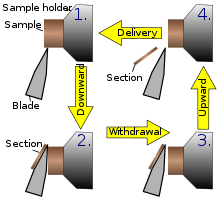
\includegraphics[width=0.40\textwidth]{chapter_4_RVE_Definition/figures/Microtomeprinciple.png}
    \caption{Microtome principle}
    \label{fig:Microtomeprinciple}
\end{figure}
% https://en.wikipedia.org/wiki/Microtome

These pieces have a thickness that is thin enough to have light transmitted trough them, images of these samples can be observed in figure \ref{fig:mesostructure} and figure \ref{fig:Meso10&20}. Since there is no microtome available at the TU Delft or TNO an alternative method was developed. The samples where printed out of a ABS grade provided by Ultimaker \cite{TechnicalUM}. 

The goal of cutting the sample was to obtain a cross-section of the part that is flat enough to perform optical microscopy without altering the material of the part. The first approach was to create a notch with a razor blade attached to a UTS machine before freezing the part in liquid nitrogen and break it with an impact test machine. This resulted unsuccessful, since the part shattered in multiple shards and only created ruptures in between the roads (the desired cross section surface is an perpendicular intra-road cut). After examining the resulting shards, the surface of the notch seemed relatively clean and smooth. After analyzing this surface with an optical microscope, the micrographs showed significant overlap with the microtomed samples. 

To validate this method, results of a sample analyzed with Computer Tomograhpy (CT) were compared with a FFF produced part by the DDDrop \cite{VeenEnhancingTemperature} in PETG which was cut with a UTS machine with a razor blade that is normally used to notch polymer specimen. The rate of cutting was kept low (2mm/min) to minimize the plastic deformation and allow the polymer to "creep" around the blade. The results are presented in figure \ref{fig:CTOM} and seemed to have a large degree of coherence with the results of the CT scan. Images from the the OM results were compared with the CT scan on a point that is in relative proximity (<5mm) in the axial direction. A particular point in the cross section of both images seemed to overlap in shape and position. Even if the location has not been fully verified, the image of the OM show a large enough overlap with the CT cross section and the micrographs of the literature (\ref{fig:mesostructure} and \ref{fig:Meso10&20})) to assume that this method produces relevant micrographs to determine the mesostructure and road structure.  

Therefore, it can be concluded that the method applied with the cutting of a sample through a UTS machine with a razor can generate relevant cross-sectional images that represent the mesostructure. 

\begin{figure}[H]
    \centering
    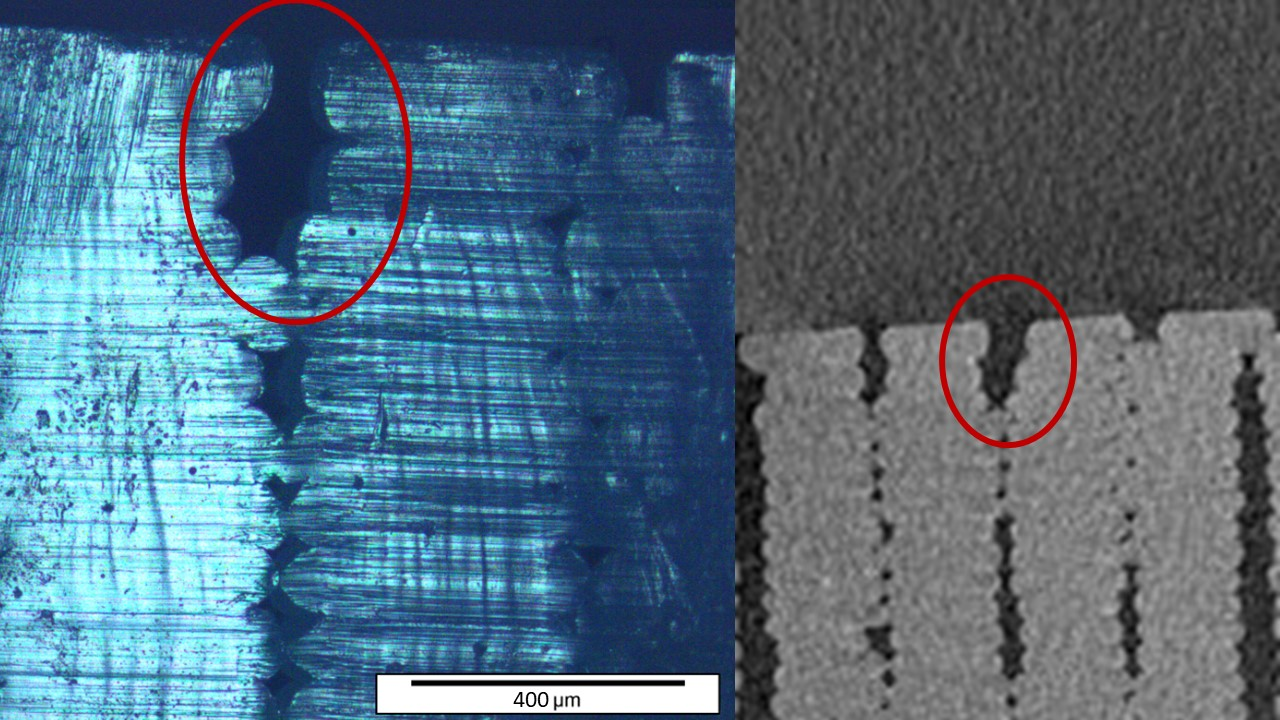
\includegraphics[width=0.4\textwidth]{chapter_4_RVE_Definition/figures/CTOM.jpg}
    \caption{Optical Microscopy (left) and CT (right) \cite{VeenEnhancingTemperature}}
    \label{fig:CTOM}
\end{figure}

The method that is used for the cutting of cross-sectional parts has therefore been defined as follows; a part produced according to table \ref{tab:parameters} is cut by a UTS machine (\ref{tab:hardware}) with a razor blade used for polymer notching at a compression rate of 2mm/min. The part is placed on a wooden frame base plate, and is cut with >1mm offset from the bottom.

\subsection{Production strategy}
The used production parameters and hardware are defined in table \ref{tab:parameters}. As is discussed in chapter 2,  high speed has a negative effect on the mechanical properties, therefore an appropriately low speed was used to produce the samples.

\begin{table}[h]
	\allign
	\caption{Parameters for cross sectional analysis}
	\label{tab:parameters}
	\begin{tabular}{ll}
		%	\begin{tabularx}{0.8\columnwidth}{XX}
		Parameter  &     \\
		\hline
		Line thickness & 0.2 mm \\
		Line width & 0.4 mm \\
		Speed & 35 mm/s \\
		Flow multiplier & 100\% \\
		Printing temperature & 230 C\textdegree \\
		Bed temperature & 85 C\textdegree \\
		Thickness beam & 4 mm \\
		Width beam & 10 mm \\

		\hline
	\end{tabular}
	%	\end{tabularx}
\end{table}

\begin{table}[h]
	\centering
	\caption{Hardware specification}
	\label{tab:hardware}
	\begin{tabular}{ccc}
		%	\begin{tabularx}{0.8\columnwidth}{XX}
		Type  & Hardware & Software    \\
		\hline
		FFF system & Ultimaker S5 & Cura 4.0 \\
		UTS system & Zick/Roell z010 10kN & Test Expert \\
		Optical Microscope & CHECK! & CHECK! \\		
        Digital Microscope & plugable usb 2.0 digital microscope & plugable digital viewer \\
		Computational Tomography & Phoenix nanotom CT  & phoenix datos|x CT \\

	

		\hline
	\end{tabular}
	%	\end{tabularx}
\end{table}

A part was produced in the YX[0] and analysed to determine the form and amount of porosity in the sample. Additionally a bi-chromatic YX[0] sample was analysed to observe the bonding between roads. The print strategy for the bi-chromatic sample is shown in \ref{fig:colorroads}. The slicer software is not able to define different types of filament for a resolution smaller than 4 roads. 

\begin{figure}[H]
    \centering
    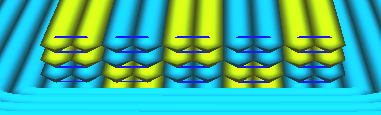
\includegraphics[width=0.4\textwidth]{chapter_4_RVE_Definition/figures/colorroads.PNG}
    \caption{CURA visualization of the road structure}
    \label{fig:colorroads}
\end{figure}

The dual head of the UM S5  allows to deposit alternating black and white roads. The extruding system is configured to deposit all roads of a type consecutively in a layer, this effect alternates between layers. This phenomenon alters the road structure slightly in comparison with single filament parts. Since the goal is to identify the adhesion and geometry of the deposited roads, the above mentioned phenomenon needs to be taken into account.

\section{Microscopy}
The used optical microscope  (\ref{tab:hardware}) has a default magnification of 10 and has a lens revolver with minimum magnification of 5. This would result in a magnification of 50, which would give an image of about 3 by 5 roads with the current process parameters.
Since the micrographs with a magnification of 50 do not include the whole cross-sectional surface area, a set of points across the specimen where observed. This is also done to observe the effect of the razor blade on the sample.
To achieve an image of the whole cross sectional area a digital microscope was used. The image produced with this microscope allows a larger view of the image.

%\subsection{Effect of flow modifier on mesostructure} maybe later
%To identify the effect of the flow modifier (which is similar to the modification of the negative airgap as is discussed in chapter \ref{chp:lit_rev}), a cross-sectional analysis was performed with parts produced with different flow modifiers. Cross sections with flow modifiers of 90\% up to 110\% with increments of 5\% where analyzed under a optical microscope. Most micrographs are produced with the lowest magnification (50), since this gives a good overview of multiple connected roads. Some micrograhps implement a larger magnification, these will be pointed out in the results. 

%Additionally, the surfaces (top, sides and bottom) are relevant to determine the degree of distortion related to the increase of the flow multiplier, this is especially relevant for the top surface, since the accumulated material will mostly stack in the z-direction. Also, the bottom will currently show a deformed stated of the material, since it is teared up manually. Not being that relevant for the current subject, it is still interesting to observe the behaviour of the material and mesostructure under plastic deformation.

%\subsection{Volume fraction based on archimedes principle}
%LATER archimedes principle, part should be large enough to determine well. 

\section{Results}
The results of the optical microscopy are presented in figure \ref{fig:Mesoresults} and \ref{fig:ABS100yxmiddle}. 

\subsection{Optical micrographs mesostructure regular analysis}

\begin{figure}
\centering
  \begin{subfigure}[b]{0.48\textwidth}
  \centering
    \includegraphics[width=\textwidth]{chapter_4_RVE_Definition/figures/ABS100middle.png}
    \caption{Picture 1}
    \label{fig:1.0}
  \end{subfigure}
  %
  \begin{subfigure}[b]{0.48\textwidth}
    \includegraphics[width=\textwidth]{chapter_4_RVE_Definition/figures/ABS100bottomcorner.png}
    \caption{Picture 2}
    \label{fig:2}
  \end{subfigure}
  \\
    \begin{subfigure}[b]{0.48\textwidth}
    \includegraphics[width=\textwidth]{chapter_4_RVE_Definition/figures/ABS100top.png}
    \caption{Picture 3}
    \label{fig:3}
  \end{subfigure}
  %
  \begin{subfigure}[b]{0.48\textwidth}
    \includegraphics[width=\textwidth]{chapter_4_RVE_Definition/figures/ABS100topcorner.png}
    \caption{Picture 4}
    \label{fig:4}
  \end{subfigure}
  \\
  
  \caption{Mesostructure of different positions, produced according to table \ref{tab:parameters}. (a) middle, (b) left bottom, (c) top, (d) left top}
    \label{fig:Mesoresults}
\end{figure}

In figure \ref{fig:Mesoresults} images of different region of the mesostructure of are shown. Different regions of the surfaces are shown (top, sides and bottom).

\begin{figure}[H]
    \centering
    \includegraphics[width=0.50\textwidth]{chapter_4_RVE_Definition/figures/ABS100yxmiddle.png}
    \caption{Fractured surface observed with optical microscopy}
    \label{fig:ABS100yxmiddle}
\end{figure}

In the figure \ref{fig:ABS100yxmiddle} a fracture cross section is showed after a specimen was subjected to a tensile test. The image is blurred due to the rough failure surface.

\subsection{Optical micrographs mesostructure colored analysis}

The results of the optical microscopy of the colored analysis are shown in figure \ref{colored roads}. and \ref{colored roads 500x zoom}. As can be seen, these roads alter in color according to figure \ref{fig:colorroads}. 
\begin{figure}
\centering
  \begin{subfigure}[b]{0.48\textwidth}
    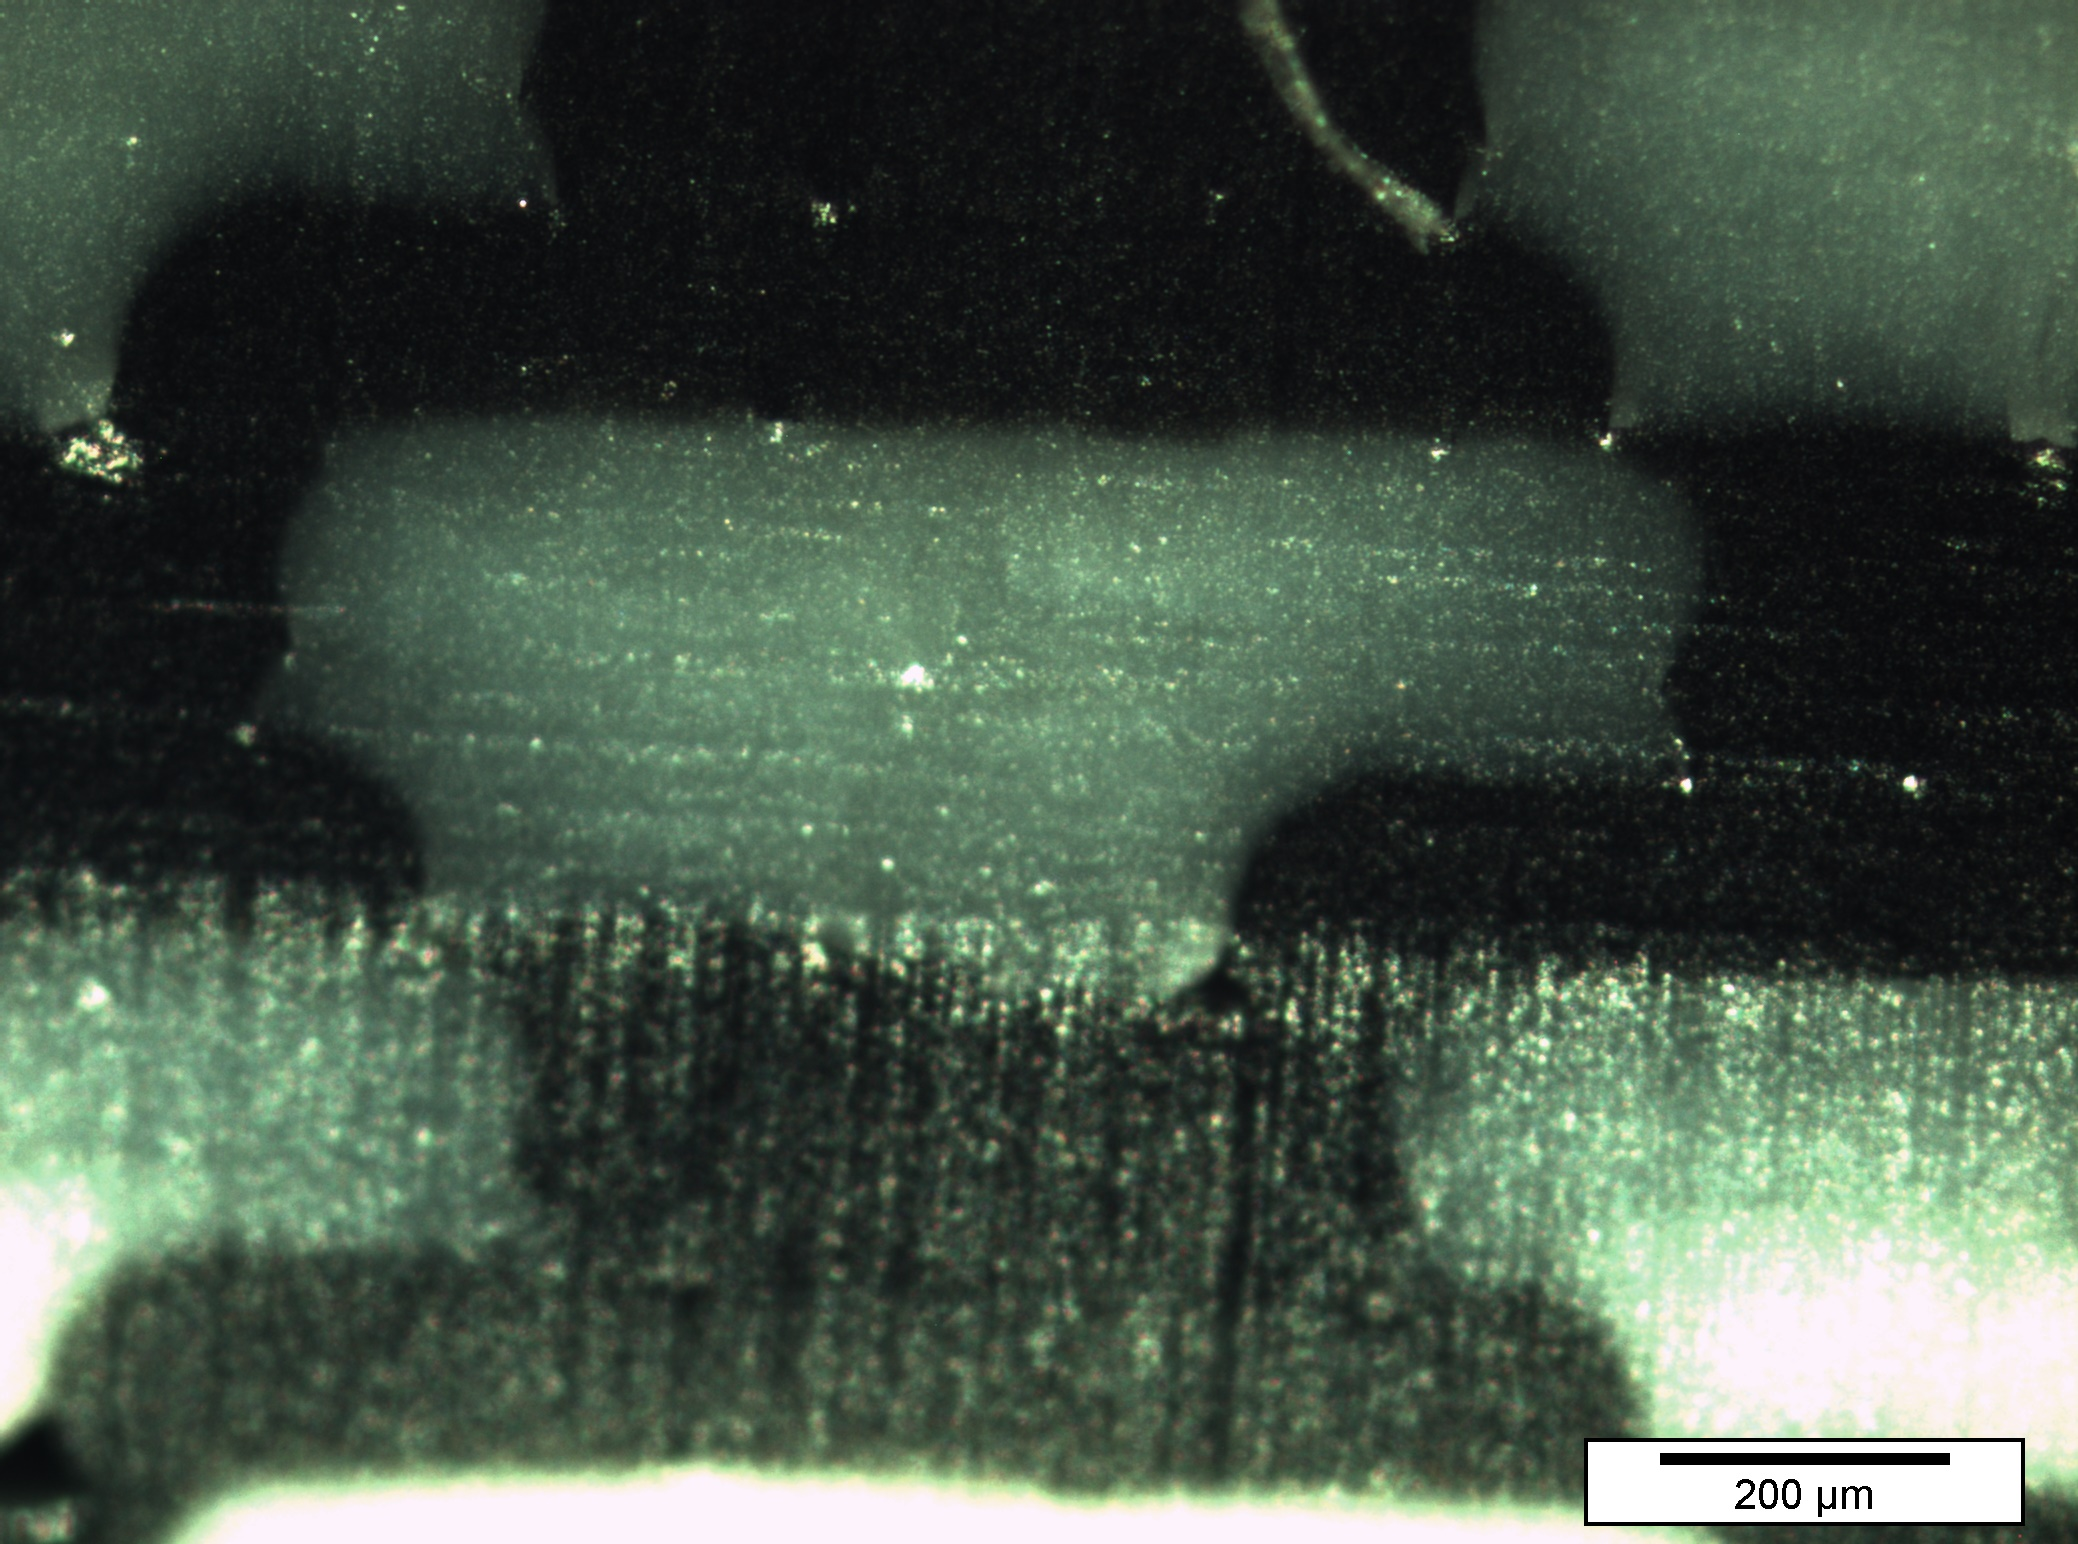
\includegraphics[width=\textwidth]{chapter_4_RVE_Definition/figures/colored/Tv35_LI.jpg}
    \caption{Picture 1}
    \label{fig:1}
  \end{subfigure}
  %
  \begin{subfigure}[b]{0.48\textwidth}
    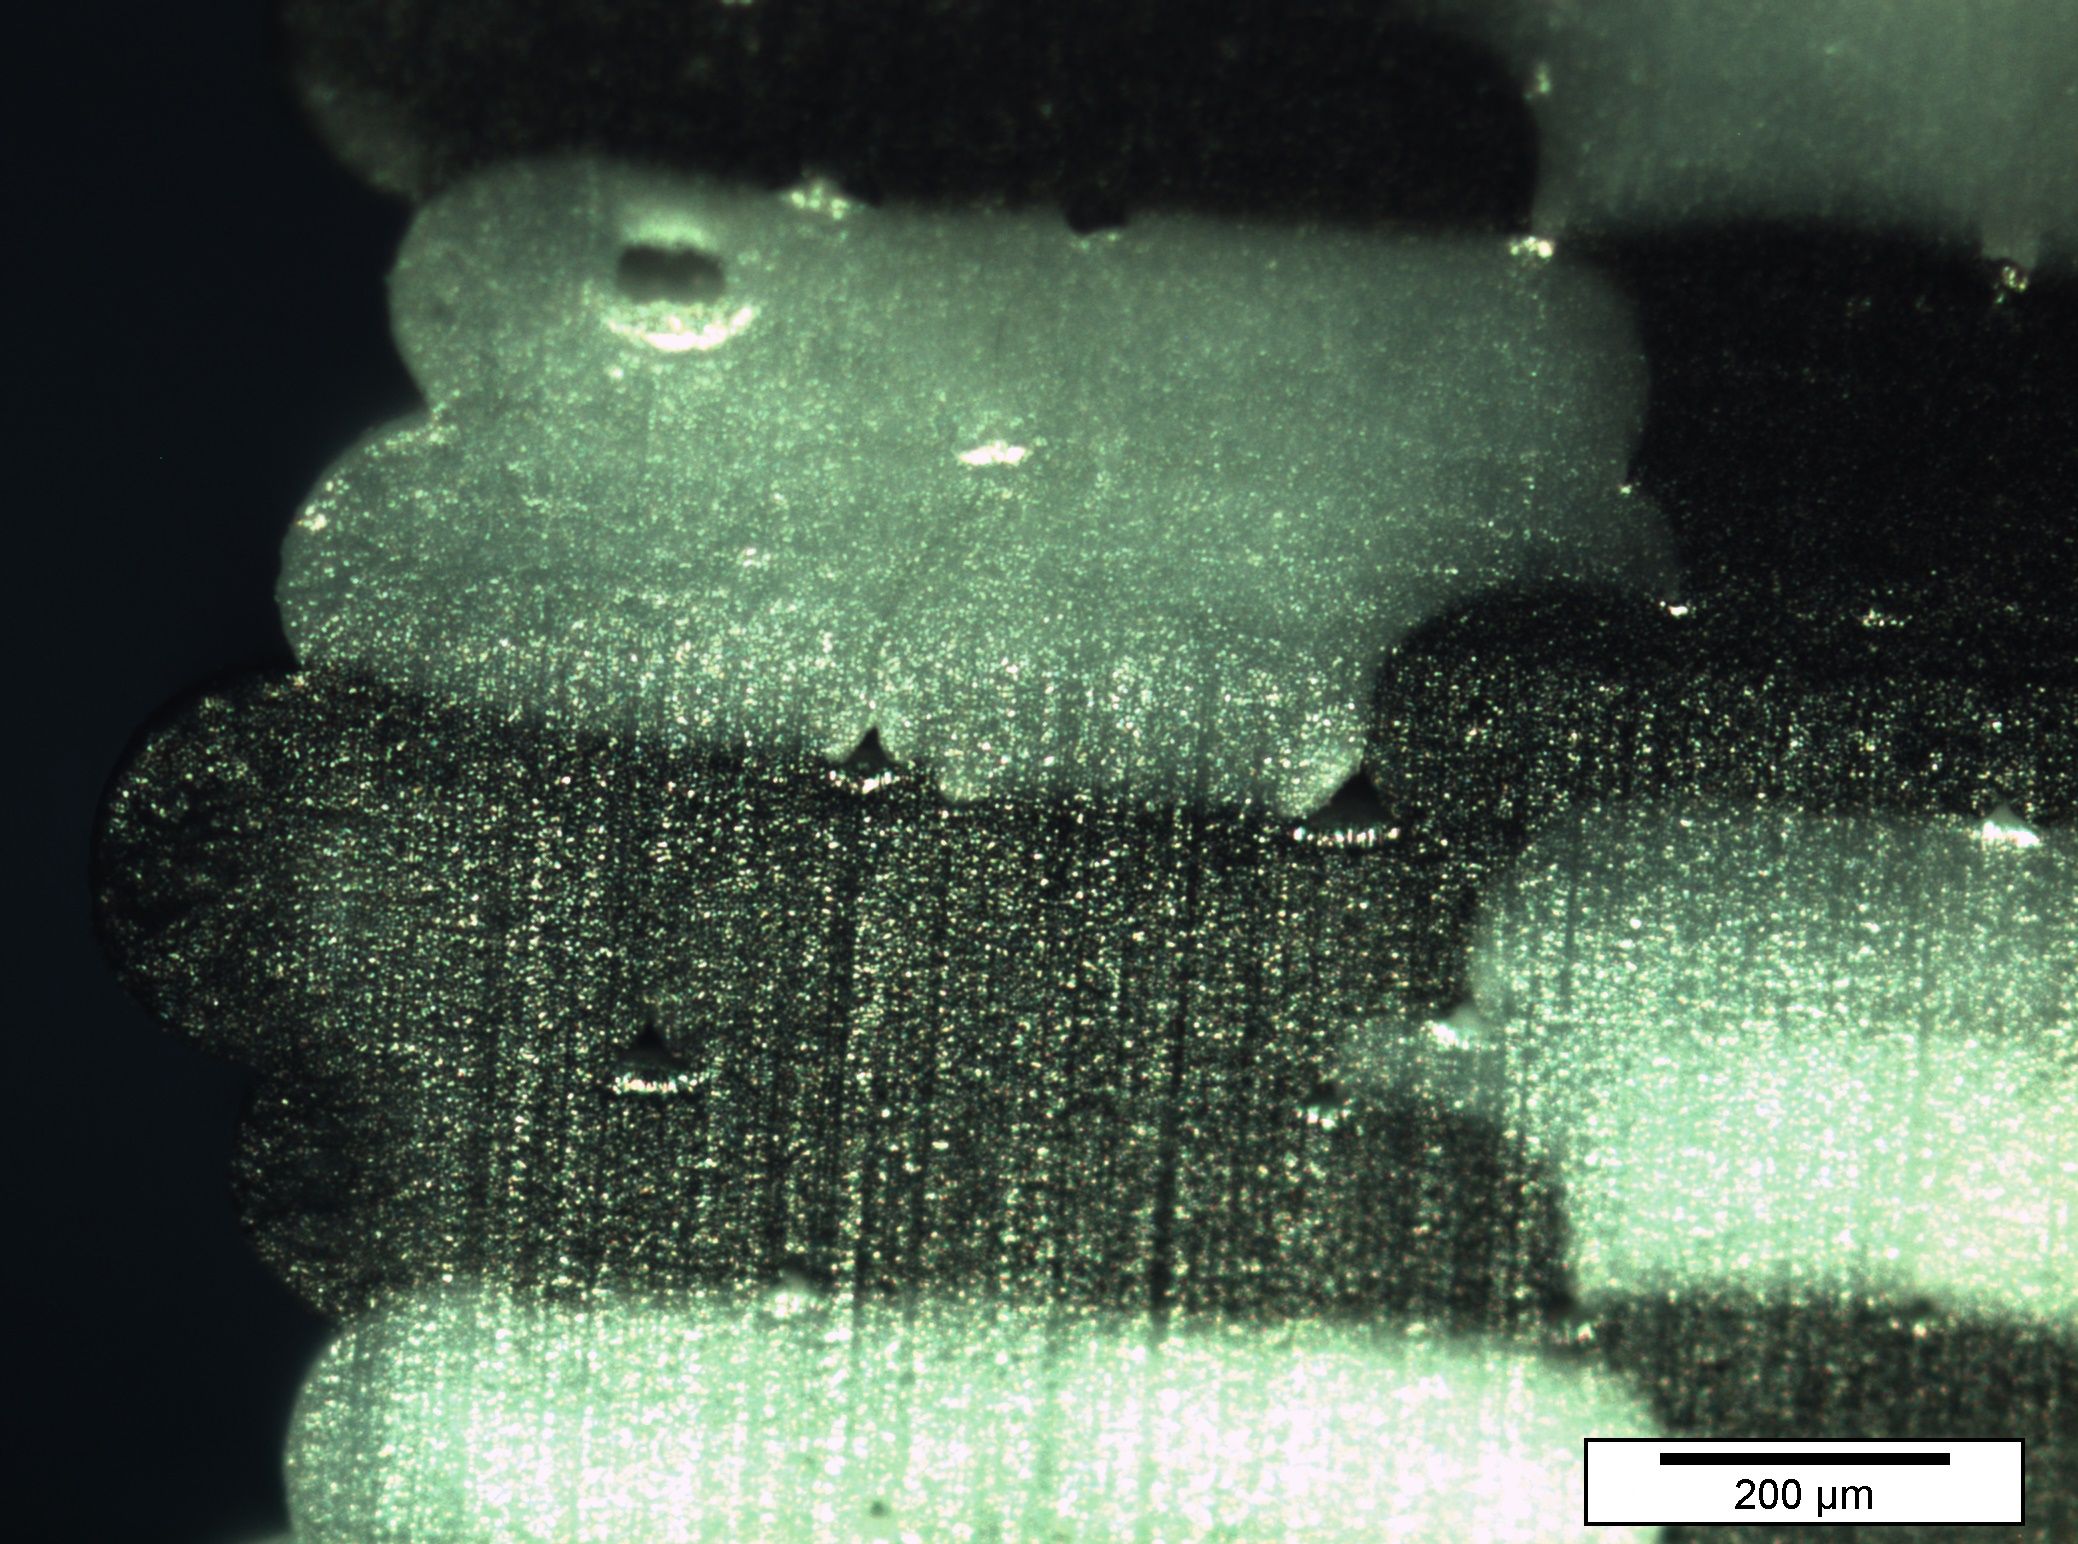
\includegraphics[width=\textwidth]{chapter_4_RVE_Definition/figures/colored/Tv38_LI.jpg}
    \caption{Picture 2}
    \label{fig:2}
  \end{subfigure}
  \\
    \begin{subfigure}[b]{0.48\textwidth}
    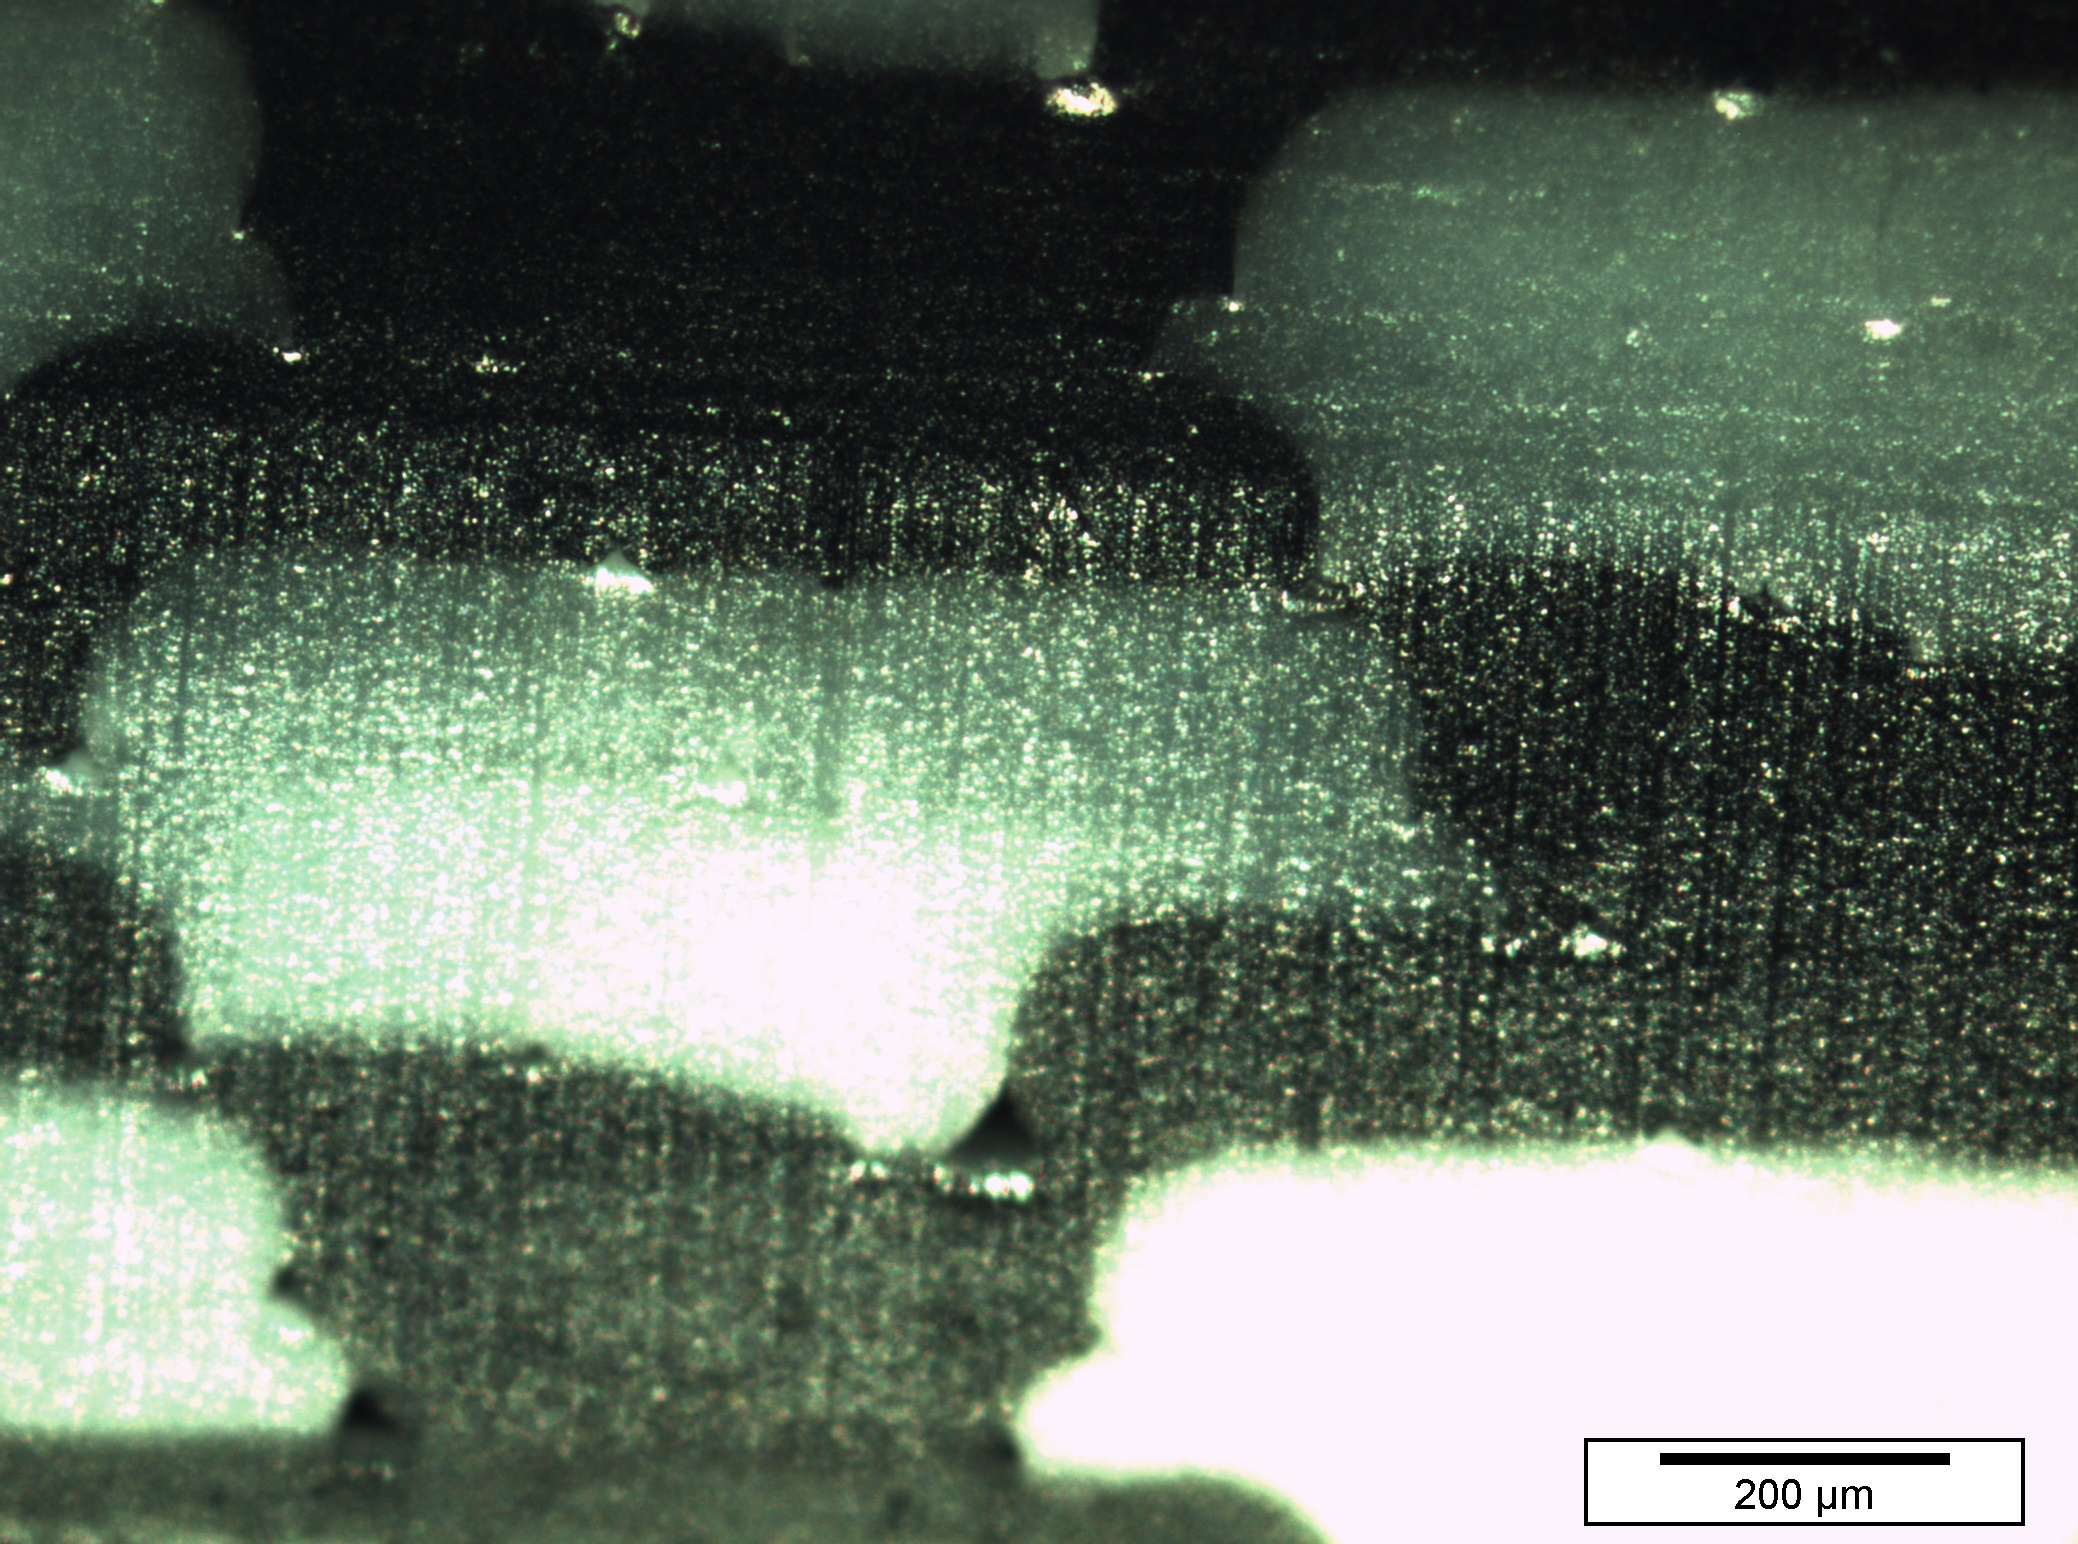
\includegraphics[width=\textwidth]{chapter_4_RVE_Definition/figures/colored/Tv42_LI.jpg}
    \caption{Picture 3}
    \label{fig:3}
  \end{subfigure}
  %
  \begin{subfigure}[b]{0.48\textwidth}
    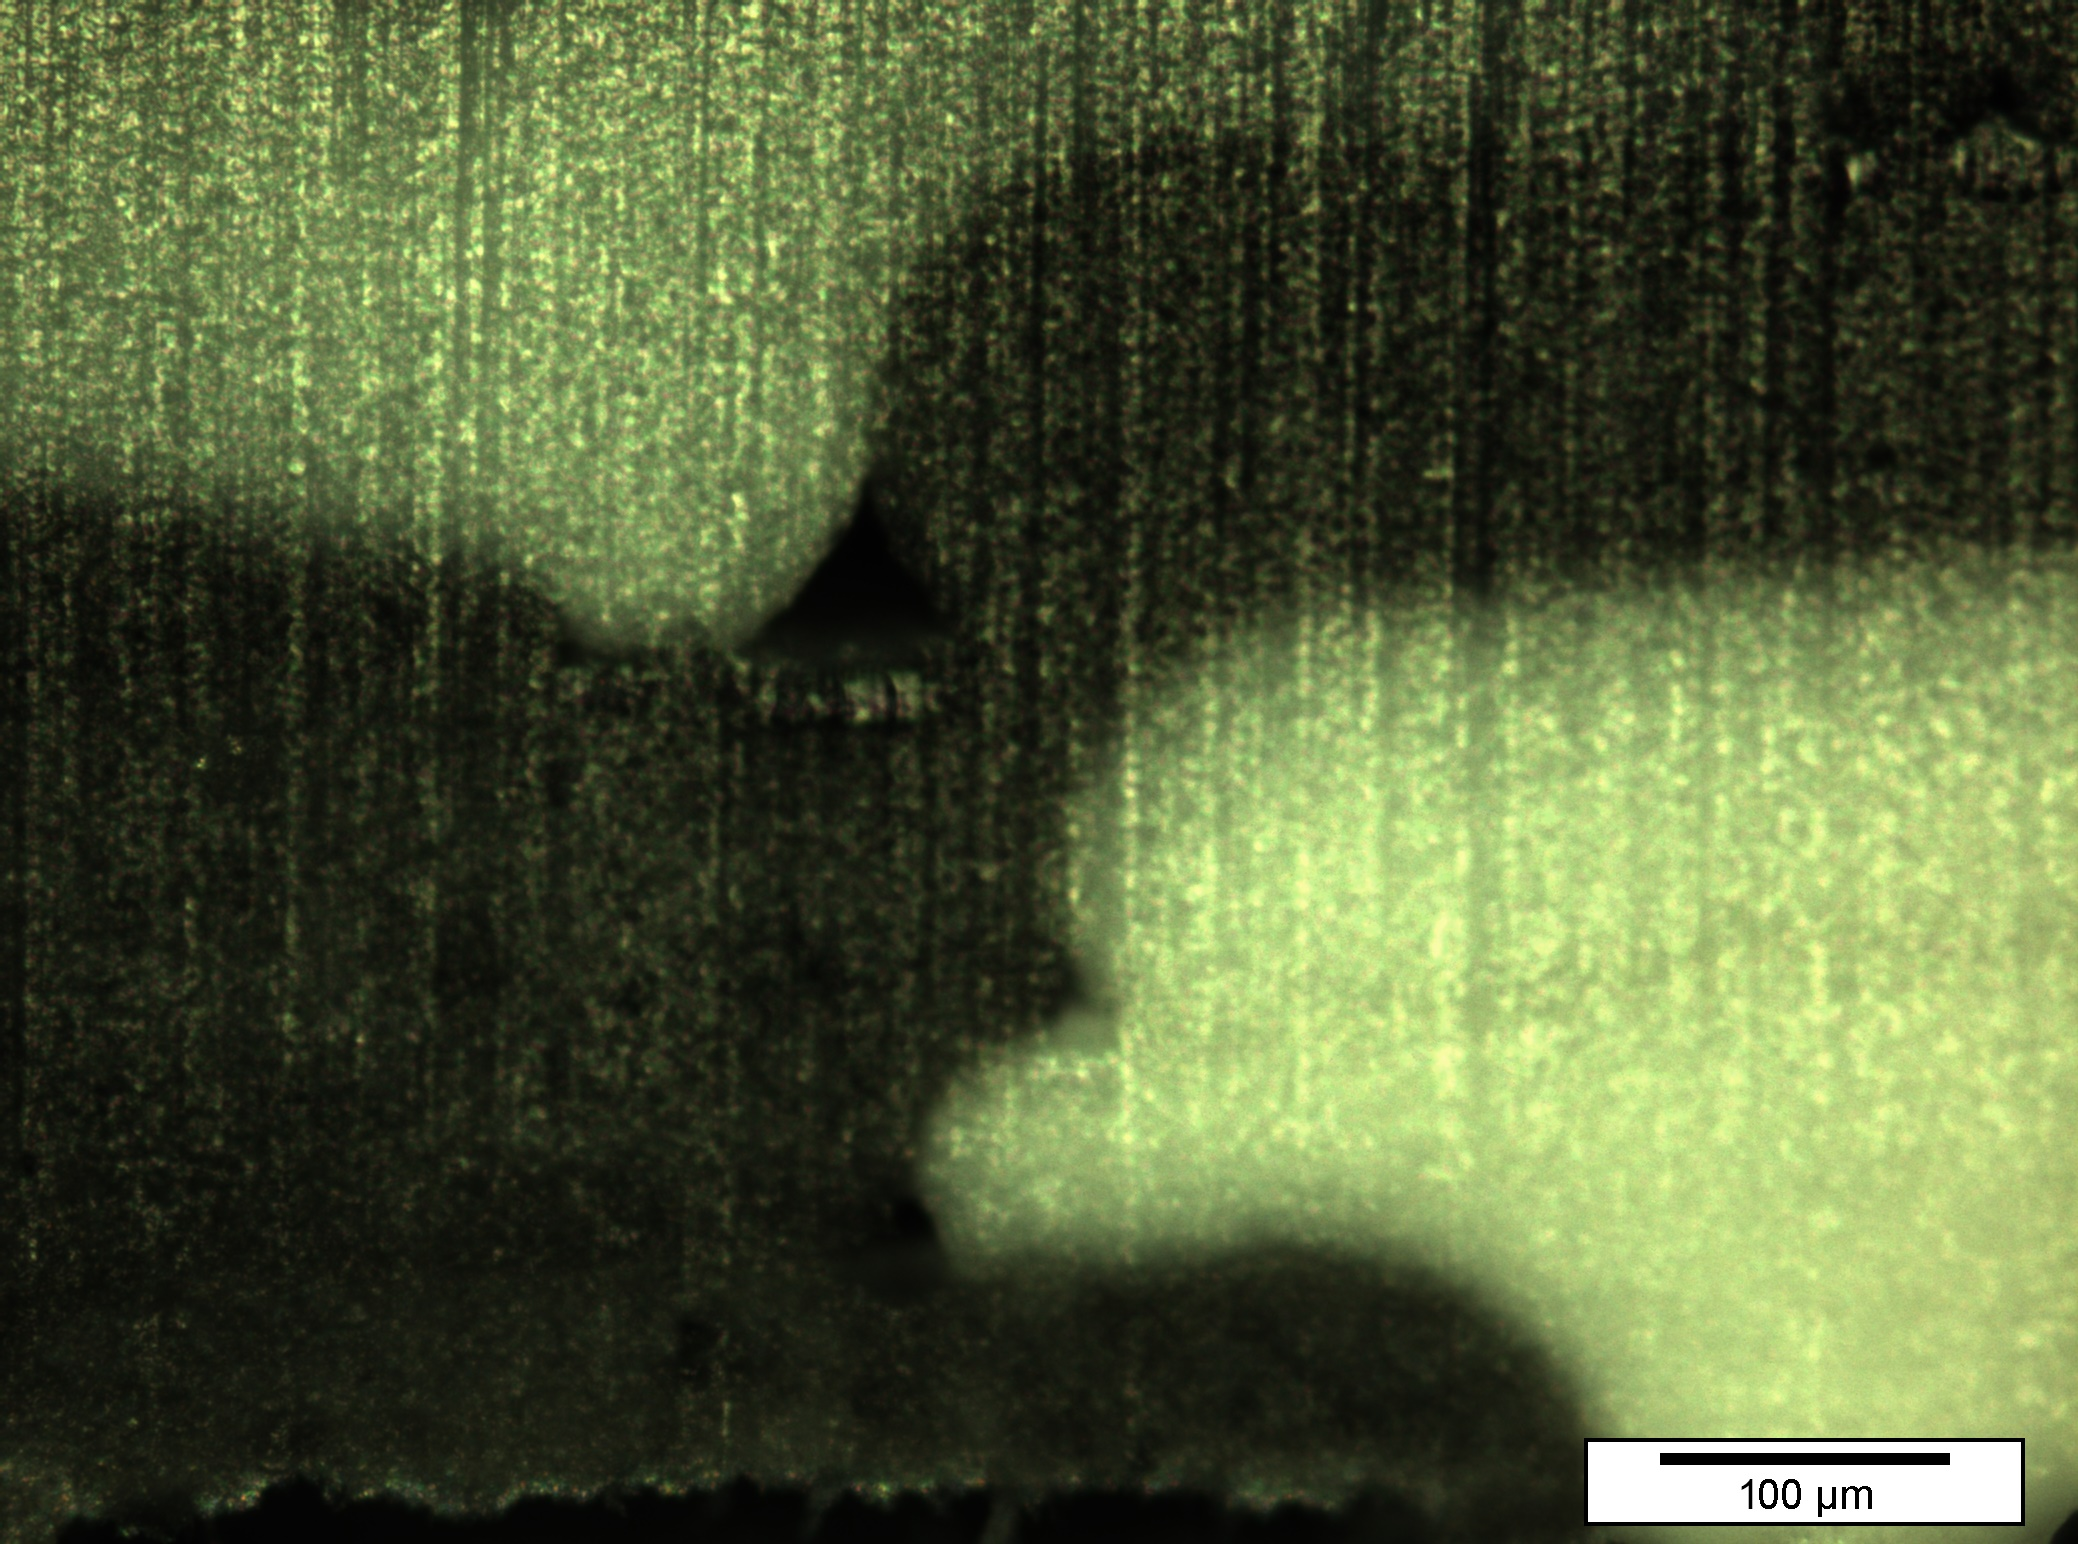
\includegraphics[width=\textwidth]{chapter_4_RVE_Definition/figures/colored/Tv86a_LI.jpg}
    \caption{Picture 4}
    \label{fig:4}
  \end{subfigure}
  \\
  
  \caption{Cross sectional mesostructure of the colored roads at different positions. }
    \label{fig:Colored roads}
\end{figure}

Figure \ref{fig:colored road 500x zoom} shows a 500x zoom on a road interface to observe the weld between different roads.
\begin{figure}[H]
    \centering
    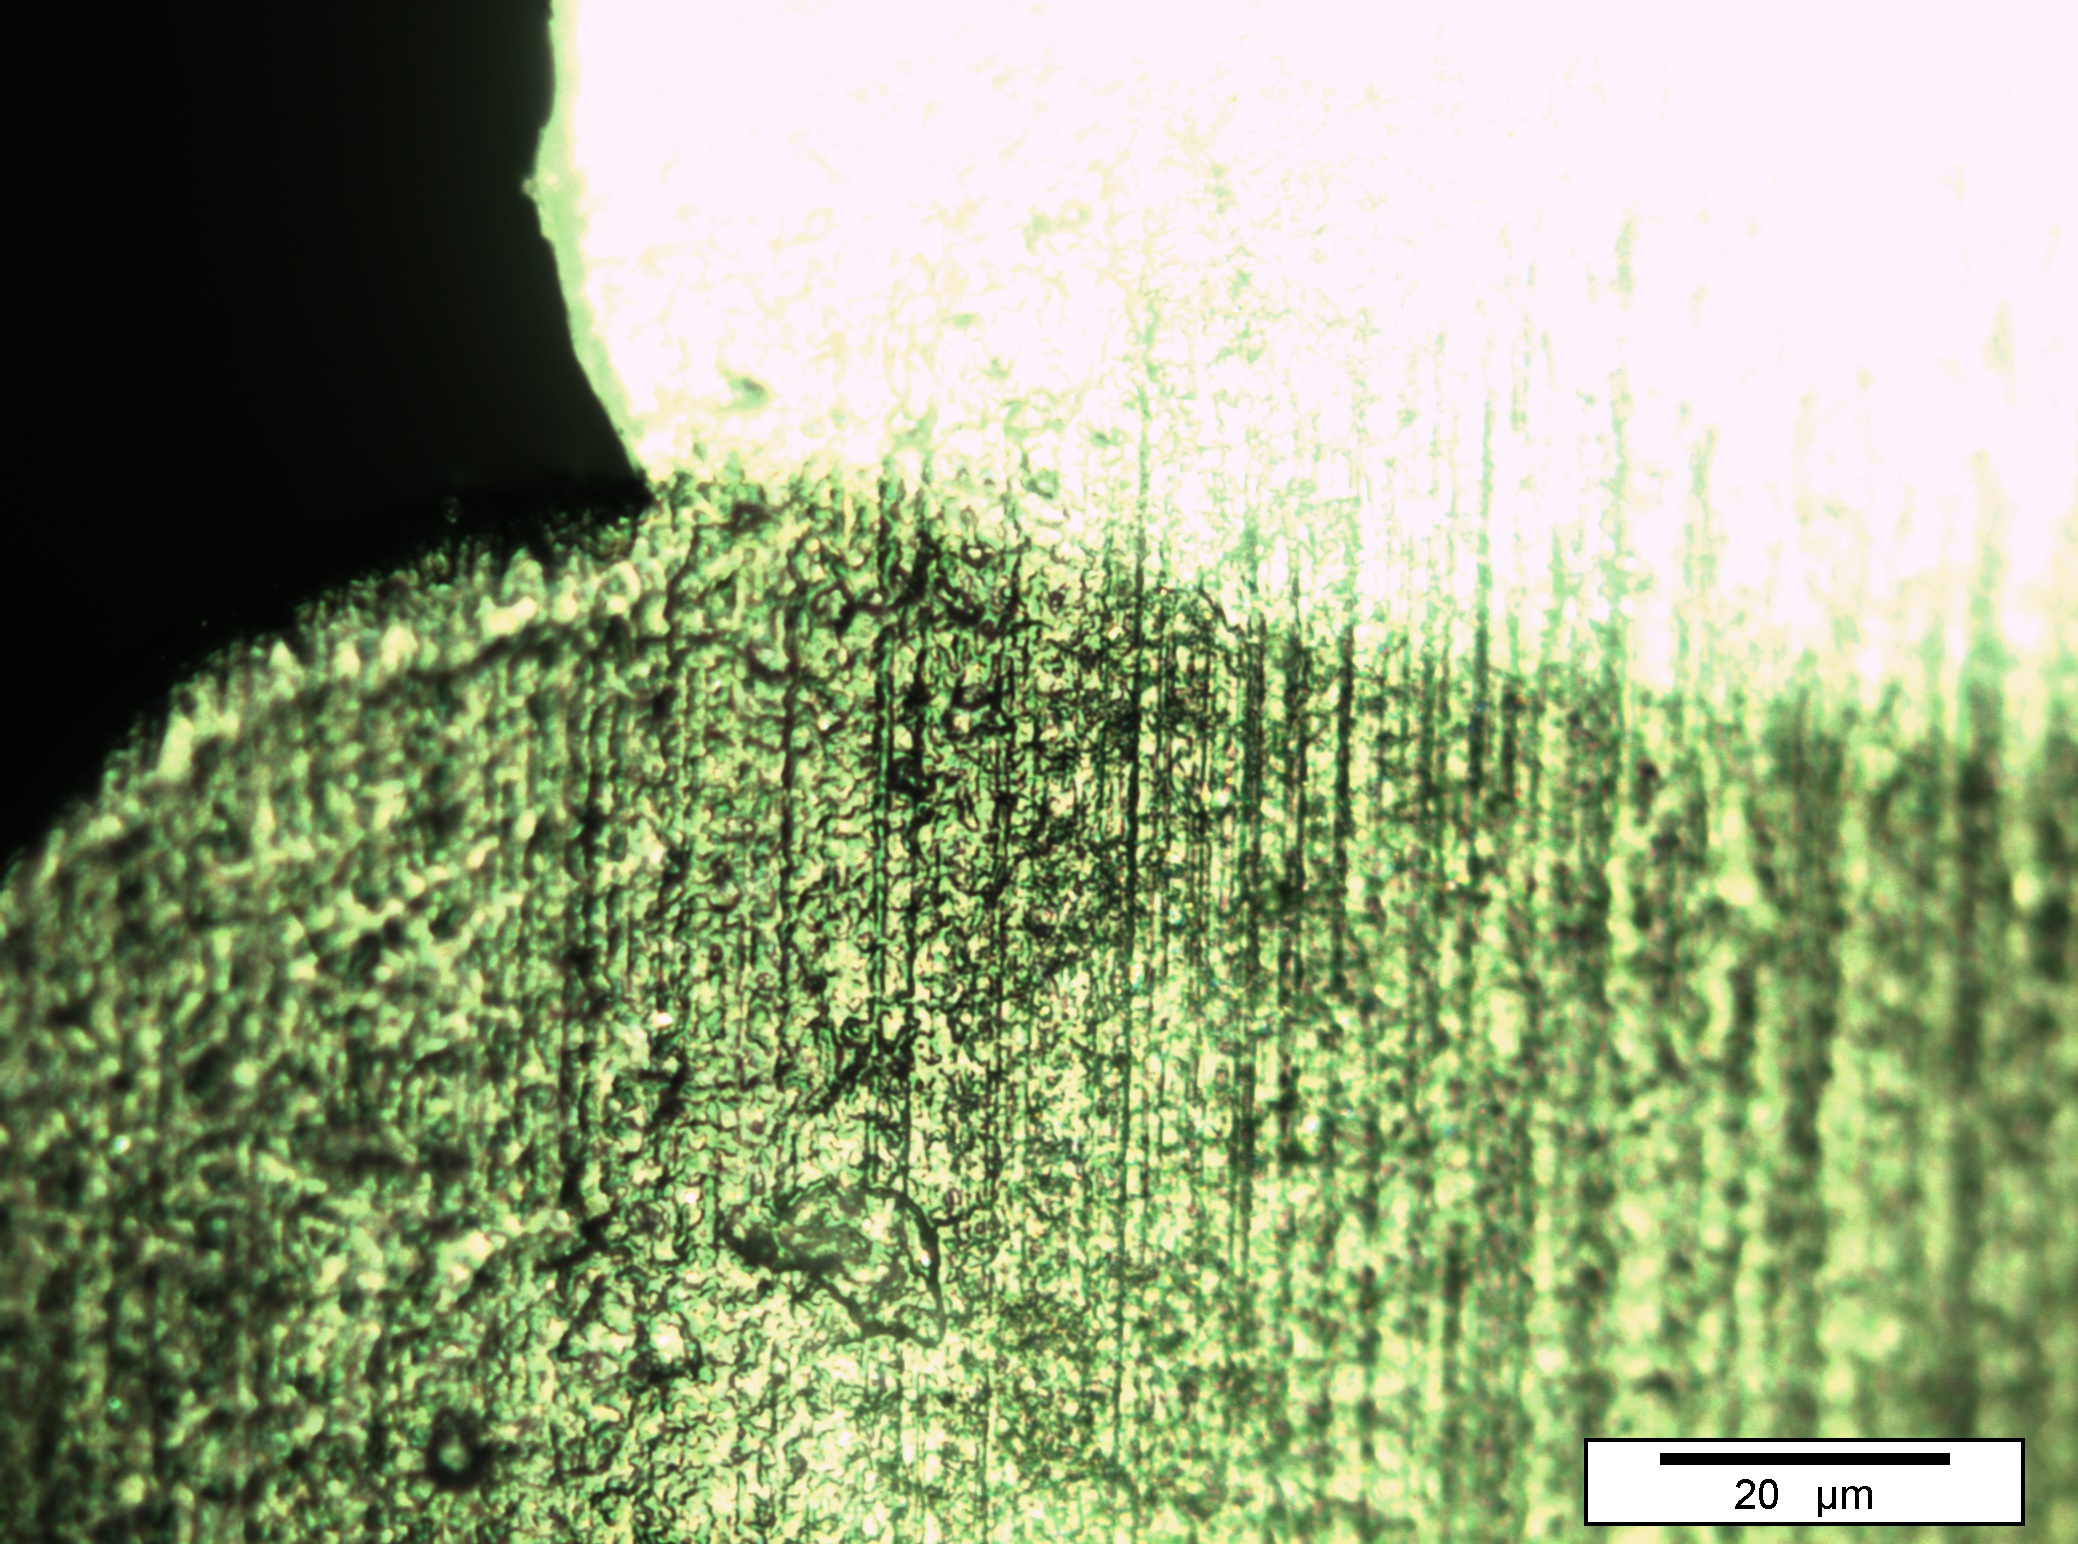
\includegraphics[width=0.40\textwidth]{chapter_4_RVE_Definition/figures/colored/Tv89_LI.jpg}
    \caption{Road interface 500x zoom}
    \label{fig:colored road 500x zoom}
\end{figure}

\subsection{Digital micrographs  mesostructure colored analysis}

In figure \ref{digitalcolored} a larger cross section of the colored roads is shown.
\begin{figure}[H]
    \centering
    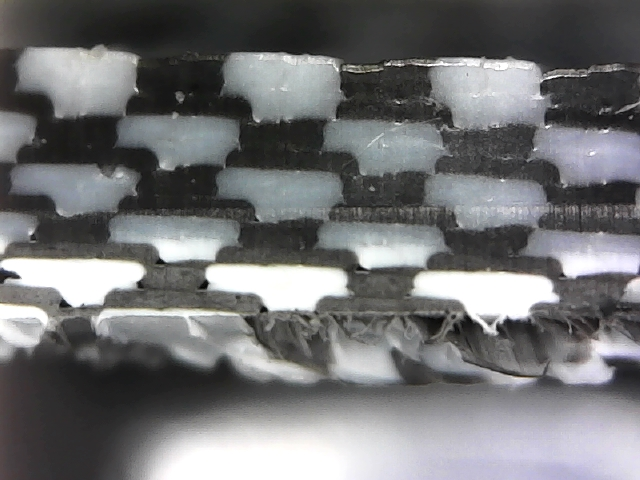
\includegraphics[width=0.40\textwidth]{chapter_4_RVE_Definition/figures/colored/Digitalcolored.jpg}
    \caption{Digital microscopy of the colored road analysis}
    \label{fig:digitalcolored}
\end{figure}

\section{Discussion}

%//Micrographs do not overlap with literuature
In the investigated micrographs (figure \ref{fig:Mesoresults}) it can be clearly seen that the porosity is significantly different from the mesostructures defined by the literature, figures \ref{fig:mesostructure} and \ref{fig:Meso10&20}. The porosity of Somireddy, figure\ref{fig:Meso10&20}, exhibits a diamond shape. In the porosity analyzed by Rodriguez \ref{fig:mesostructure} a more triangular cavity is observed. The SEM pictures of Ahn, figures \ref{fig:AhnMeso} and \ref{fig:SEMmesostructure}, show a different form, where the cavities are quite large and the form is shaped like a four armed star. Other micrographs, e.g. presented by Li \cite{Li2002CompositeProperties} show a reversed triangle as porosity. The differences in porosity suggest a strong dependency on  process hardware and process parameters.

%// meso is triangles instead of stars
The produced micrographs have triangular shaped cavities, which is clearly seen in figure \ref{fig:2} and figure \ref{fig:ABS100yxmiddle}. Figures \ref{fig:1}, \ref{fig:3}, \ref{fig:4} have a particular form, resembling dots. The pressure of the cutting knife could have deformed the mesostructure significantly. Another explanation might be explained by the accumulation of material towards the top, reducing the porosity in its way. 

%//theory on porosity filling
Since the slicers are  modeled to create a certain percentage of overlap (5-10\%), pushing the roads closer together, some of the material of the extruded road is "pushed" on top of the road next to it. This eliminates the the porosity of the top corner (the side next to the adjacent road) of the road that is being extruded. This theory is in line with the observed results, which show a lack of porosity which exactly matches the before mentioned effect. 

%//information of the sides and top
The sides of the specimen show clear curvature of the molten roads. The spots between the curvatures are potential stress concentration points, which will be discussed in chapter 5.
On the top the mono-chromatic sample (figure \ref{fig:Mesoresults} (c) and (d)) there seems to be a certain amount of distortion (wave like artifacts), this can be accounted to the theory of overlap between roads. Additionally, the nozzle can create nicks in the roof by passing too close to the surface.

%// colored roads
The multicolored specimen with black and white filament was produced to investigate the interfaces between road. The figures \ref{fig:Colored roads} and \ref{fig:digitalcolored} are cross sectional micrographs of these multi-colored specimen, these show a significantly less structured mesostructure in comparison to the mono-chromatic specimen. This is likely due to the sequence of deposition; a type of filament is consecutively deposited in one layer,  ensuing squeezing of the second type between roads due to the programmed road overlap. This phenomenon largely influences the density and the contact surface between roads, resulting in better mechanical properties.

%// information on road structure according to slicer
The theory of the larger line width which causes overlap is supported by a slicer producer called "Slic3r" \cite{GaryHodgsonSlic3rMath}. One of the programmers of Slic3r explains how the line width is calculated based on the porosity that needs to be filled. They assume that roads are extruded in rectangular shape with  semicircular ends as can be seen in figure \ref{fig:Slic3rshape.png}, this shape is generally referred to as "stadium shapes".

\begin{figure}[H]
   \centering
    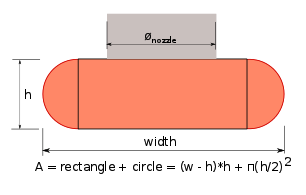
\includegraphics[width=0.40\textwidth]{chapter_2/figures/Slic3rshape.png}
    \caption{Road geometery according to Slic3r \cite{GaryHodgsonSlic3rMath}}
    \label{fig:Slic3rshape}
\end{figure}

The height of these roads is defined by $l_h$, the distance between roads is defined by $l_w$. The ratio between these two is presented as $R=(l_h/l_w)$.
These roads have a certain "extruded width", which is a function of line height $l_h$ and line width $l_w$ according to equation \ref{eqn:extrudedwidth} and are deposited with a certain distance relative to the center of the adjacent road which is equal to the line width. 

\begin{equation} \label{eqn:extrudedwidth}
e_w=l_w+l_h\cdot(1-\pi/4)
\end{equation}
This creates a certain "overlap" defined as $\Delta l$, earlier defined as "negative airgap", which is defined by equation \ref{eqn:overlap}. Slic3r calculates this overlap in the "line width" based on the porosity that the geometry of the roads would generate to be filled up with the overlap surface. In figure \ref{fig:Roadoverlapslic3r} the yellow area represents the void area to be filled. If the roads where to deposited closer to eachother, an overlapped surface will emerge, which ideally would generate enough overlap to fill up both voids. He proposes an overlap factor (from 0 to 1) to find the optimum for filling in the void area's, the overlap factor represents how much void remains between the extrusions. It's difficult to estimate this amount, since it also depends on viscosity of plastic, extrusion speed and temperature. In the this discussion we will assume the $\Delta l$ to generate an overlap to fill both the cavities. 
If the road is deposited next to the adjacent road from the top, it is very unlikely that the bottom void is filled. To be sure that there is abundant material available to fill these voids, the line width is still defined based on a equal surface of void and overlap area. A similar process has been presented by Sun, Li and Bellehumeur \cite{Li2002CompositeProperties} but results in a reversed triangle which is not in agreement with our micrographs. Tronvoll et al. \cite{TronvollTheApproach} explain the same phenomenon in a recently published article.


\begin{figure}[H]
    \centering
    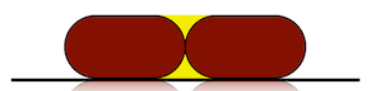
\includegraphics[width=0.40\textwidth]{chapter_4_RVE_Definition/figures/Roadoverlapslic3r.PNG}
    \caption{Road overlap according to Slic3r \cite{GaryHodgsonSlic3rMath}}
    \label{fig:Roadoverlapslic3r}
\end{figure}
The overlap $\Delta l$ between roads is defined as the difference between extruded width $e_w$ and line width $l_w$

\begin{equation} \label{eqn:overlap}
\Delta l=e_w-l_w
\end{equation}

%A different approach is followed by the Slic3r manual written by Hodgson \cite{GaryHodgsonSlic3rMath} where he explains how the extruded material of the roads is calculated. In his model he assumes a stadium shaped road, which is also supported by Patanwala \cite{Patanwala2018TheComposites} Additionally to the conclusions found in the section about road width, Hodgson claims that with a higher line width the bonding in the z direction would be better due to a larger contact area and consequently a lower amount of porosity. 
%If we follow the defintion of Hodgson, the road structure can be defined by two parameters in the slicer, the line width $l_w$ (distance between deposited roads) and layer height $l_h$. In reality other process parameters such as speed, flow rate and temperature also alter the road structure, for this analysis we assume these to be constant and to have minor effect on the resulting layer height and line width.

%The extruded roads will have a geometric shape that reassembles mostly a stadium shape. The height of this road is the layer height $l_h$, and the width is the extruded line width $e_w$.

%The extruded line width $e_w$ is dependent on the layer height $l_h$ and layer width $l_w$ with the following relation. 

For a line ratio of 0.5, the $\Delta l$ is equal to 0.043, which is in line with the observations in literature, among other Somireddy, who observed a 10\% overlap. The line ratio is recommended to be around 0.5, and is not recommended to surpass 1.  In figure \ref{fig:Roadstructure2} the resulting RVE is presented.
%In this geometry two voids are generated, the upper void will be filled by the deposited material while it is still in a semi-molten state. The result is a road geometry that has a periodic triangular porosity. The resulting road structure can be observed in figure \ref{fig:Roadstructure2}

\begin{figure}[H]
    \centering
    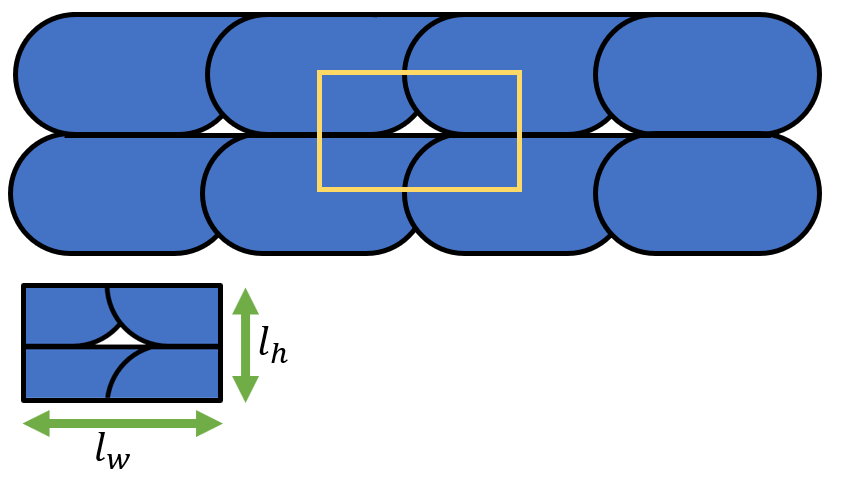
\includegraphics[width=1\textwidth]{chapter_4_RVE_Definition/figures/Roadstructure2.PNG}
    \caption{New defined road structure}
    \label{fig:Roadstructure2}
\end{figure}

The area of a road is subsequently calculated with is calculated as following: 
\begin{equation} \label{eqn:crazecriterion}
A_{road}=(e_w-l_h)*l_h+\pi(l_h/2)^2
\end{equation}
And the area of the RVE with the simple relation between line width and line height:
\begin{equation} \label{eqn:crazecriterion}
A_{RVE}=l_h*l_w
\end{equation}
%diameter, the excess line width (which was expected to be 10\% by Somireddy) becomes 50\%(!). The micro graphs and single lines produced are in line with the 10\% theory, however the tolerance tests gave results that the parts to be fitted have a over dimension of 0.3-0.4 in 2 directions, resulting in a 75\%-100\% increase in line width, which would actually be closer in line with the Hodgson theory.

Now that the form of the RVE is defined by the $l_h$ and $l_w$ parameters, we can define a relation of the void surface according to: 
\begin{equation}
A_v = ((l_h/2)-(e_w-l_w)/2)^2*(l_h/2)-(asin((l_h/2)-(e_w-l_w)/(l_h))/(2*\pi)*(l_h/2)^2*\pi 
\\ & &
-\sqrt{(l_h^2-((l_h/2)-(e_w-l_w)/2)^2 )}*(l_h/2)-(e_w-l_w)/2 )*2
\end{equation}
And the surface fraction of the RVE can be found with
\begin{equation}
f_v = \frac{A_v}{A_{RVE}}
\end{equation}
With this information, we can identify the surface fractions in different directions as a function of the line ration. The surface fraction of the 1 direction is straightforward, for the 2 and 3 directions it is more tricky since the cavity is not consistent in these directions. As is assumed by Li and Rodriguez, we can identify the largest void fraction in the cross section as can be seen in figure \ref{fig:Surfacefraction}.

\begin{figure}[H]
    \centering
    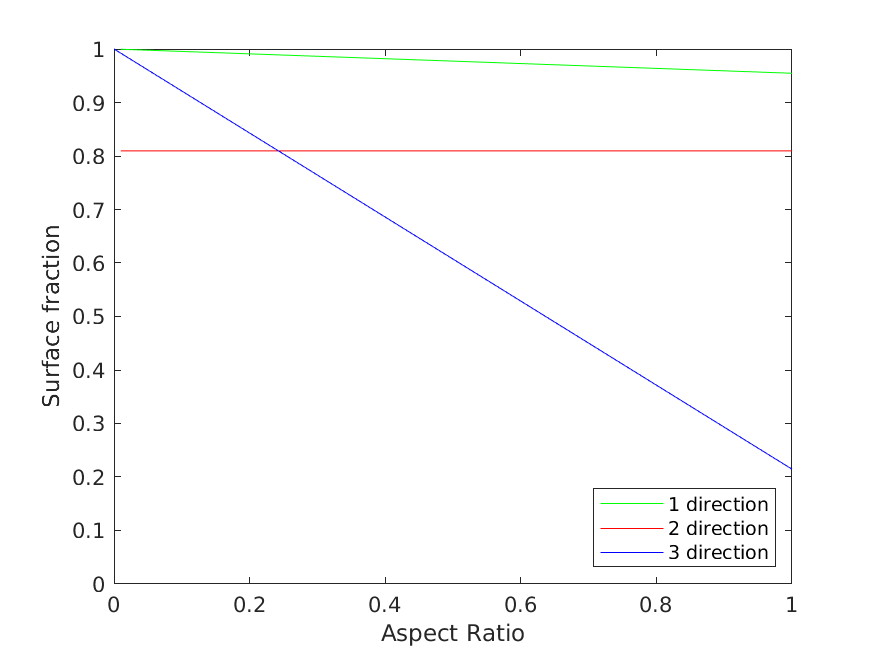
\includegraphics[width=0.5\textwidth]{chapter_4_RVE_Definition/figures/Surfacefraction.png}
    \caption{Surface fraction of RVE vs line ratio}
    \label{fig:Surfacefraction}
\end{figure}

The RVE's with ratio 1 and 1/8 are shown in figures \ref{fig:RVE1} and \ref{fig:RVE1/8}.
\begin{figure}[H]
    \centering
    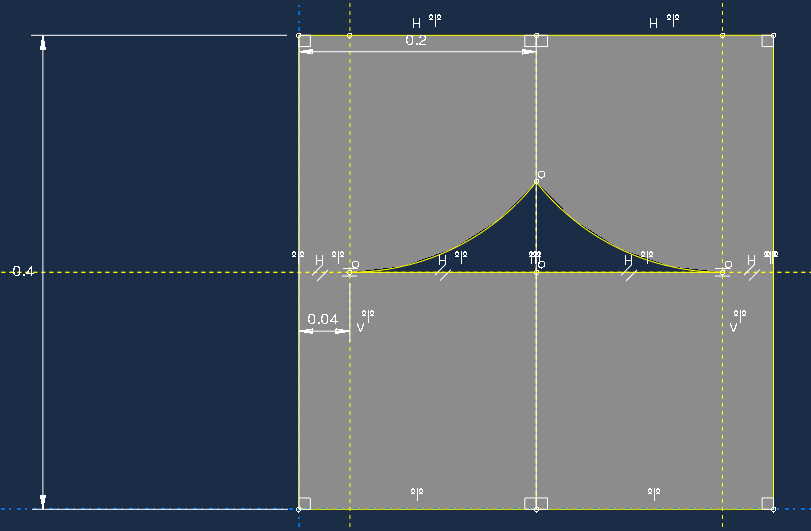
\includegraphics[width=0.5\textwidth]{chapter_4_RVE_Definition/figures/RVER1.png}
    \caption{RVE with a ratio of 1}
    \label{fig:RVE1}
\end{figure}

\begin{figure}[H]
    \centering
    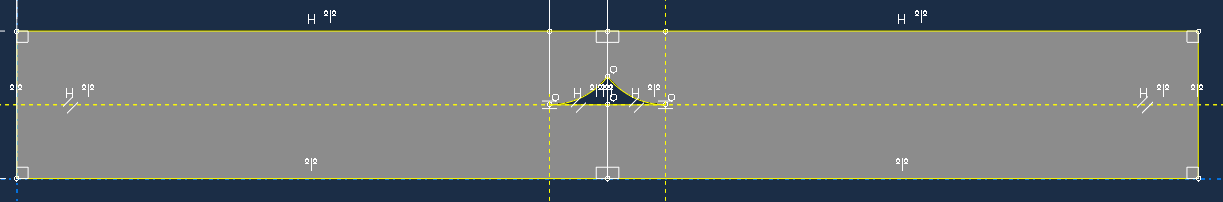
\includegraphics[width=0.5\textwidth]{chapter_4_RVE_Definition/figures/RVER8.png}
    \caption{RVE with a ratio of 1/8}
    \label{fig:RVE1/8}
\end{figure}


%%%% PARTLY DISCUSSION ON COLORED ROADS


%%% RVE definition
\subsection{Conclusion}
With the information gathered from the literature, generated micrographs and slicer information a geometry can be defined that corresponds with our hardware and process parameters. The obtained micrographs show the same periodicity that can be found in the micrographs from the literature, additionally, it corresponds with the theory provided by Hodgson. In literature no good definition was given for this phenomenon, mainly due to the fact that different FFF systems produce a variety of mesostructures. 
With these definitions an RVE can be defined that is dependent on the line width and line height, the surface of the cavity can be predicted based on these parameters. Now that we have model that can predict the volume, shape and location of the porosity, analytical and numerical models can be implemented to determine the effect of this mesostructure. 

In appendix A a derivation of the road deposition is presented to substantiate our theory. 

%\\further research
This road structure can be used as an RVE in further analysis. It should be investigated whether the results with this mesostructure definition is in line with the experimental results for specific line width and height parameters.

%\section{Degree of bonding} LATER
%\subsection{Degree of bonding}LATER Optical bonding with differ

%\section{Results}

%\section{Analysis of road structure}

%\subsection{Analysis of road structure}

%\subsection{Analysis of Flow}


%\section{RVE analysis}
%\subsection{Determination of the RVE form}
%\subsection{Determination of the young's modulus}
%\subsection{Determination of failure criterion}

%\section{Mechanical experimentation}
%\subsetion{Different directions}







%3. Methods, Equipment and Procedures – Describes what you have done and how
%you did it, with sufficient detail to ensure that the work can be reproduced with the
%same results by someone else with a similar educational background.


\graphicspath{{chapter_4/figures/}}
\graphicspath{{chapter_2/figures/}}% path to the figures folder of this chapter



